% Copyright (c) 2009-2015 by the University of Waikato, Hamilton, NZ.
% This work is made available under the terms of the 
% Creative Commons Attribution-ShareAlike 3.0 license, 
% http://creativecommons.org/licenses/by-sa/3.0/. 
%
% Version: $Revision: 3363 $

\documentclass[a4paper]{book}

\usepackage{wrapfig}
\usepackage{graphicx}
\usepackage{hyperref}
\usepackage{multirow}
\usepackage{scalefnt}
\usepackage{tikz}
\usepackage{varwidth}

% watermark -- for draft stage
\usepackage[firstpage]{draftwatermark}
\SetWatermarkLightness{0.9}
\SetWatermarkScale{5}

\hyphenation{ImageMagick}
\hyphenation{ImageJ}

% Copyright (c) 2009 by the University of Waikato, Hamilton, NZ. 
% This work is made available under the terms of the 
% Creative Commons Attribution-ShareAlike 3.0 license, 
% http://creativecommons.org/licenses/by-sa/3.0/. 
%
% Version: $Revision$

\newenvironment{tight_itemize}{
\begin{itemize}
  \setlength{\itemsep}{1pt}
  \setlength{\parskip}{0pt}
  \setlength{\parsep}{0pt}}{\end{itemize}
}

\newenvironment{tight_enumerate}{
\begin{enumerate}
  \setlength{\itemsep}{1pt}
  \setlength{\parskip}{0pt}
  \setlength{\parsep}{0pt}}{\end{enumerate}
}

% if you just need a simple heading
% Usage:
%   \heading{the text of the heading}
\newcommand{\heading}[1]{
  \vspace{0.3cm} \noindent \textbf{#1} \newline
}

\newcommand{\icon}[1]{\tikz[baseline=-3pt]\node[inner sep=0pt,outer sep=0pt]{\includegraphics[height=1.1em]{#1}};}


\title{
  \textbf{ADAMS} \\
  {\Large \textbf{A}dvanced \textbf{D}ata mining \textbf{A}nd \textbf{M}achine
  learning \textbf{S}ystem} \\
  {\Large Module: adams-imaging-imagej} \\
  \vspace{1cm}
  
\includegraphics[width=2cm]{images/imaging-imagej-module.png} \\
}
\author{
  Peter Reutemann
}

\setcounter{secnumdepth}{3}
\setcounter{tocdepth}{3}

\begin{document}

\begin{titlepage}
\maketitle

\thispagestyle{empty}
\center
\begin{table}[b]
	\begin{tabular}{c l l}
		\parbox[c][2cm]{2cm}{\copyright 2009-2015} &
		\parbox[c][2cm]{5cm}{
\includegraphics[width=5cm]{images/coat_of_arms.pdf}} \\
	\end{tabular}
	
\includegraphics[width=12cm]{images/cc.png} \\
\end{table}

\end{titlepage}

\tableofcontents
\listoffigures
%\listoftables


%%%%%%%%%%%%%%%%%%%%%%%%%%%%%%%%%%%
\chapter{ImageJ}
ImageJ is a public domain software suite written in Java (using AWT, opposed to
Swing which ADAMS uses) for image processing, developed at National Institutes 
of Health (\cite{imagej}).

\section{Flow}
The following ImageJ actors available:
\begin{tight_itemize}
	\item \texttt{transformer.ImageJReader} -- for reading any image file that
	JAI supports\footnote{\url{http://imagejdocu.tudor.lu/doku.php?id=faq:general:which_file_formats_are_supported_by_imagej}{}}
	and forwarding an \texttt{ImagePlusContainer} object.
	\item \texttt{transformer.ImageJTransformer} -- performs a transformation
	using an existing ImageJ transformer class on the incoming image and
	outputs another image again. ImageJ plugin filters, commands and pre-recorded
	macros can be used to perform transformations.
	\item \texttt{transformer.ImageJFeatureGenerator} -- turns an
	\texttt{ImagePlusContainer} into an \texttt{weka.core.Instance} object to
	be used in WEKA. The attaced meta-data in form of a report can be added to the
	output object as well.
	\item \texttt{transformer.ImageJReleaseAllImages} -- removes all images
	currently listed in ImageJ's batch mode list, freeing up memory.
	\item \texttt{sink.ImageJReleaseImage} -- removes the incoming image from
	ImageJ's batch mode list of images, freeing up memory.
	\item \texttt{sink.ImageJWriter} -- for writing an \texttt{ImagePlusContainer}
	to a file format that ImageJ supports. If the image type cannot be
	determined based on the extension, you can also specify which type to generate.
\end{tight_itemize}

Figure \ref{imagej-greyscale-flow} shows a
flow\footnote{adams-imaging-transform\_to\_greyscale.flow} for reading images,
turning them into greyscale using a  transformer and displaying them
side-by-side.
Figures \ref{imagej-greyscale-output-original} and
\ref{imagej-greyscale-output-grey} show original and greyscale image.

\begin{figure}[htb]
  \centering
  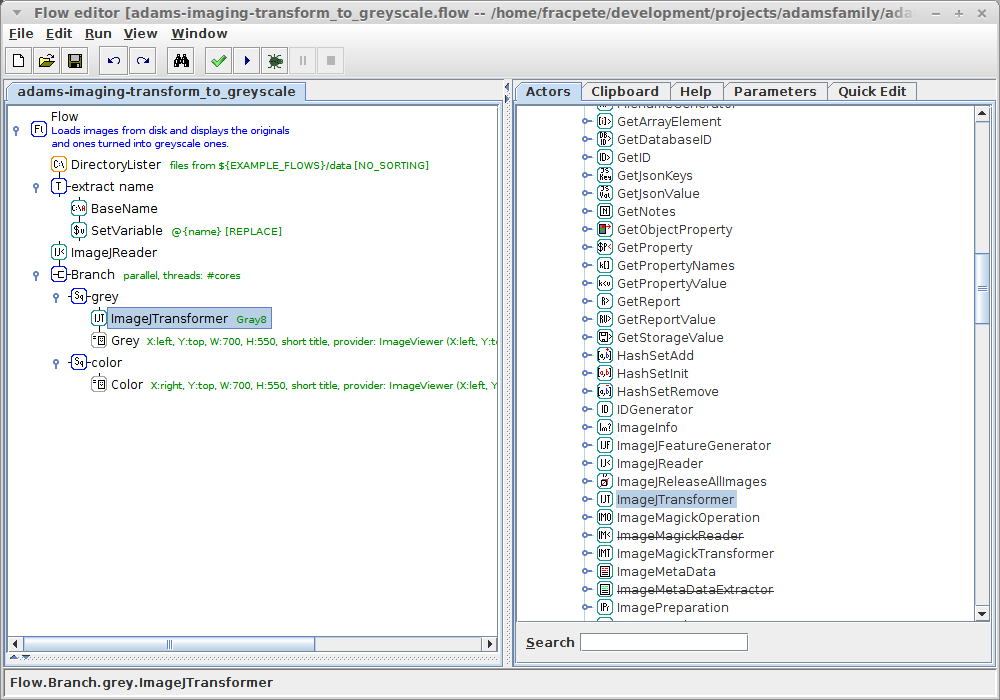
\includegraphics[width=10.0cm]{images/imagej-greyscale-flow.png}
  \caption{ImageJ flow for turning images stored in a directory into greyscale
  ones.}
  \label{imagej-greyscale-flow}
\end{figure}

\begin{figure}[htb]
  \begin{minipage}[b]{0.48\linewidth}
  \centering
  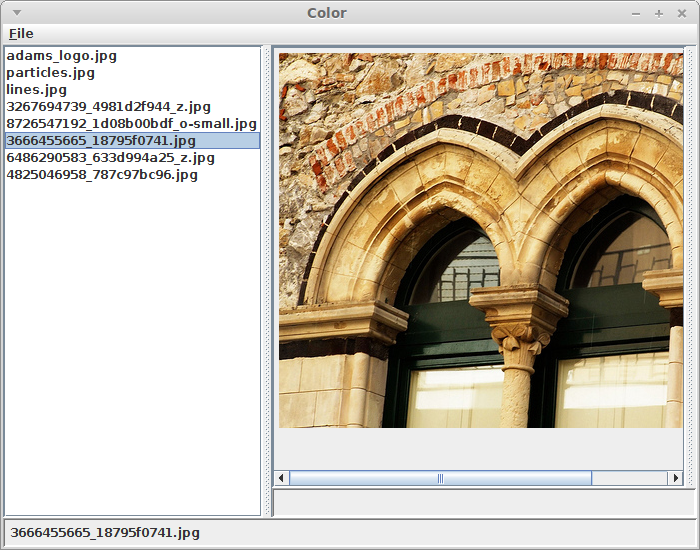
\includegraphics[height=3.7cm]{images/imagej-greyscale-output-original.png}
  \caption{The original image.}
  \label{imagej-greyscale-output-original}
  \end{minipage}%
  \begin{minipage}[b]{0.48\linewidth}
  \centering
  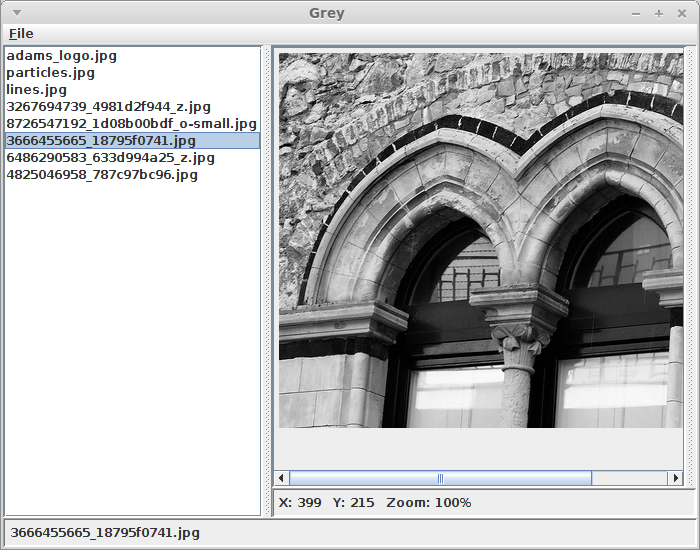
\includegraphics[height=3.7cm]{images/imagej-greyscale-output-grey.png}
  \caption{The greyscale image.}
  \label{imagej-greyscale-output-grey}
  \end{minipage}
\end{figure}

\clearpage
\section{Plugins}
By default, ADAMS includes plugins located in the following 
directory on Linux/Unix/Mac:
\begin{verbatim}
  $HOME/.adams/imagej/plugins
\end{verbatim}
and on Windows here:
\begin{verbatim}
  %USERPROFILE%/_adams/imagej/plugins
\end{verbatim}
You can override this directory by using the \texttt{ADAMS\_IMAGEJ\_DIR}
environment variable, which defines the directory one level above the 
\textit{plugins} directory. For instance, if your plugins directory is located
at:
\begin{verbatim}
  /home/user/imagej/plugins
\end{verbatim}
You have to define the \texttt{ADAMS\_IMAGEJ\_DIR} environment variable as 
follows:
\begin{verbatim}
  ADAMS_IMAGEJ_DIR=/home/user/imagej
\end{verbatim}


%%%%%%%%%%%%%%%%%%%%%%%%%%%%%%%%%%%
\chapter{Object conversion}
The following conversions are available to convert from one
format into another:
\begin{tight_itemize}
	\item \textit{ImageJToBufferedImage} -- converting from ImageJ to
	JAI/ImageMagick.
\end{tight_itemize}


%%%%%%%%%%%%%%%%%%%%%%%%%%%%%%%%%%%
% Copyright (c) 2009-2012 by the University of Waikato, Hamilton, NZ. 
% This work is made available under the terms of the 
% Creative Commons Attribution-ShareAlike 4.0 license,
% http://creativecommons.org/licenses/by-sa/4.0/.
%
% Version: $Revision$

\begin{thebibliography}{999}
	% to make the bibliography appear in the TOC
	\addcontentsline{toc}{chapter}{Bibliography}

    % references
	\bibitem{adams}
		\textit{ADAMS} -- Advanced Data mining and Machine learning System \\
		\url{https://adams.cms.waikato.ac.nz/}{}

	\bibitem{esrigrid}
	 	\textit{Esri Grid} -- a raster GIS file format deveoped by Esri. \\
		\url{https://en.wikipedia.org/wiki/Esri\_grid}{}

	\bibitem{kml}
	 	\textit{Keyhole Markup Language} -- an XML notation for expressing
	 	geographic annotation and visualization within Internet-based,
	 	two-dimensional maps and three-dimensional Earth browsers. \\
		\url{http://en.wikipedia.org/wiki/Keyhole\_Markup\_Language}{}

	\bibitem{postgresql}
	 	\textit{PostgreSQL} -- a powerful, open source object-relational
	 	database system. \\
		\url{http://www.postgresql.org/}{}

	\bibitem{postgis}
		\textit{PostGIS} -- a spatial database extender for PostgreSQL
		object-relational database. It adds support for geographic
		objects allowing location queries to be run in SQL.  \\
		\url{http://postgis.net/}{}

	\bibitem{srid4269}
	 	\textit{SRID 4269} -- or NAD 83 (North American Datum). \\
		\url{http://spatialreference.org/ref/epsg/4269/}{}

	\bibitem{mysql}
		\textit{MySQL} -- an open-source relational database management
		system (RDBMS) \\
		\url{http://www.mysql.com/}{}

\end{thebibliography}


\end{document}
